\section{Radon Transform}

Radon transformation is often used in medical imaging, e.g. computed tomography (CT). In CT data collection works by shooting x-rays through the material we try to image and collect them on the other side. If we do this from multiple angles, we can try to reconstruct an image from the measured data, as different material absorb a different amount of x-rays. We take the logarithm of this value, since absorption is a multiplicative process. \medskip

This can be seen as an image reconstruction problem.
\begin{center}
	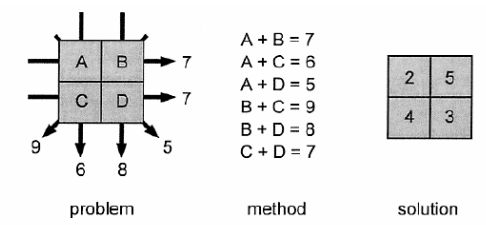
\includegraphics[width=\linewidth]{radon.png}
\end{center}

X-rays move along a straight line, at distance $s$ it has intensity $l(s)$ and after traveling $\delta s$ the intensity is reduced by $\delta l$. The reduction depends on the intensity and the optical density $u(s)$ of the material. For small $\delta s$ it holds $\delta l / l(s) = -u(s) \delta s$. This leads to the following equations:
$$I_{\text{finish}} = I_{\text{start}} \cdot e^R \qquad R = \int_L u(s)ds$$

This related to the Radon transform:
$$Rf(L) = \int_L f(x) |dx|$$

Given the following setup:
\begin{center}
	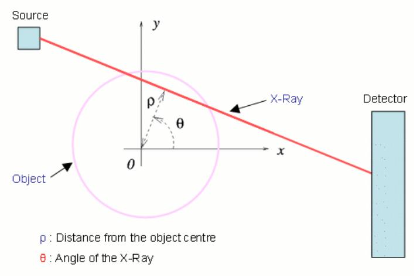
\includegraphics[width=0.8\linewidth]{data_aquisition.png}
\end{center}

We can calculate:
$$R(p, \theta) = \int_{-\infty}^\infty \int_{-\infty}^\infty u(x,y) \delta(p - x \cos \theta - y \sin \theta) dx dy$$

The Radon transform has the following properties:
\begin{itemize}
	\item Linearity
	\item Shifting only changes the $p$ coordinate
	\item Rotation of the coordinate system also rotates the Radon transformation
	\item The Radon transform of a 2D convolution is a 1D convolution of the Radon transformed function with respect to $p$
\end{itemize}

The following image shows the Radon transform of a square. We call this a \textbf{sinogram}.
\begin{center}
	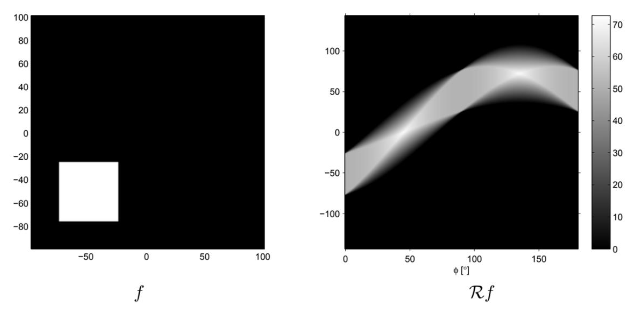
\includegraphics[width=\linewidth]{radon_square.png}
\end{center}


\subsection{Backtransformation}

Up until know we have seen how to perform a Radon transformation from an image to a sinogram. In reality we want the opposite, as medical imaging devices give us a sinogram and we want to reconstruct the image. This is the same as the question: "Can we find $u(x,y)$ if we know $R(p, \theta)$. \medskip

We can compute this with linear algebra, solving the overdetermined system $K f = g$ using normal equations. This solution is not cheap, therefore we are interested in alternative ways. One possible way of doing this would be backprojection:
\begin{center}
	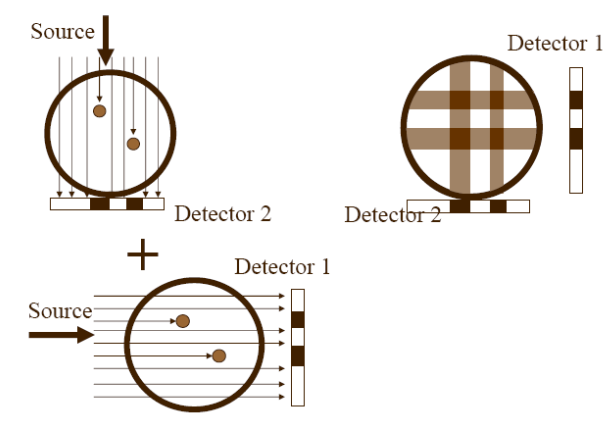
\includegraphics[width=\linewidth]{backprojection.png}
\end{center}

If we do this multiple times, adding more projections, we end up with a blurred version of the original image.

\subsubsection{Fourier / Central Slice Theorem}
$$G(q, 0) = F(q \cos 0, q \sin 0)$$

This tells us that the 1D Fourier transformation of the measurement $g = Rf$ (for a fixed $\theta$) is equal to the 2D Fourier transformation of the object slice $f(x,y)$ evaluated at a particular point. We can apply this for any orientation $\theta$.

\subsubsection{Backprojection Algorithm}
The backprojection algorithm works as follows, for each of the $K$ projection angles $\theta$:
\begin{enumerate}
	\item Measure projection data $P_\theta(t)$
	\item Fourier transform it to find $S_\theta(w)$
	\item Multiply by weighting function $2 \pi |w| / K$ (high-pass filter)
	\item Sum over the image plane and perform 2D inverse Fourier transform.
\end{enumerate}

\begin{center}
	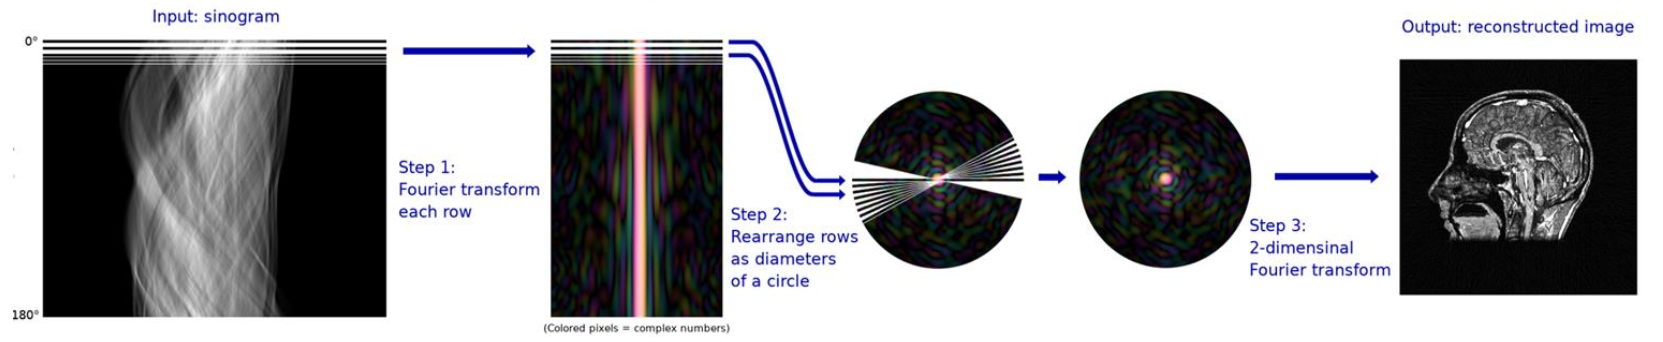
\includegraphics[width=\linewidth]{radon_fourier.png}
\end{center}

There are some practical issues, as it requires many precise measurements and is sensitive to noise it may lead to blurring in the final image.